\begin{figure}
	\begin{flushleft}
		\textbf{Login Page}:\\
		Since logging into SafeStreets is mandatory, this is the first page that the user will face when the app doesn't recognizes him. Of course, cookies or sessions could avoid to force the user to login every time.
	\end{flushleft}
	\centering
	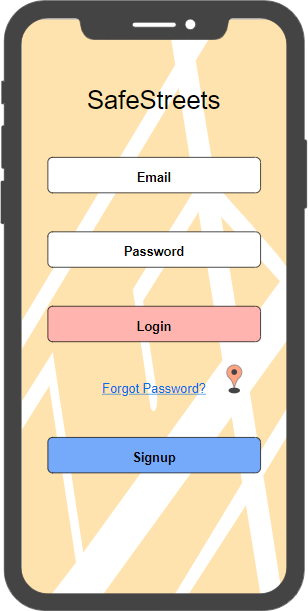
\includegraphics[width=0.6\linewidth]{images/mockups/login}
	\caption{SafeStreets Login page.}
\label{fig:login}
\end{figure}
\clearpage
\begin{figure}
	\begin{flushleft}
		\textbf{SignUp Page}:\\
		Since logging into SafeStreets is mandatory, if the user doesn't have an account he needs to make one. Every field except the photo should be obligatory.
	\end{flushleft}
	\centering
	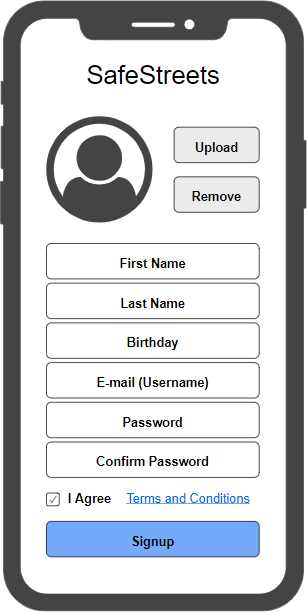
\includegraphics[width=0.6\linewidth]{images/mockups/signup}
	\caption{SafeStreets SignUp page.}
	\label{fig:signup}
\end{figure}
\clearpage
\begin{figure}
	\begin{flushleft}
		\textbf{Home Page}:\\
		When the user log into SafeStreets successfully, an home page should be provided with the options for the user to use every functionality of the application.
	\end{flushleft}
	\centering
	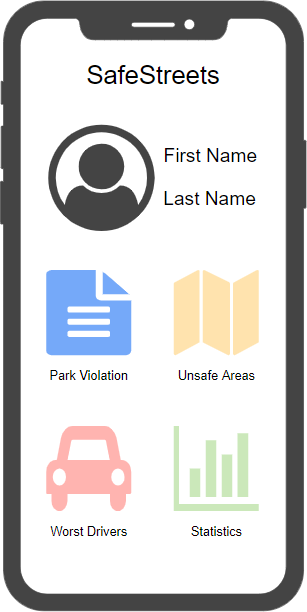
\includegraphics[width=0.6\linewidth]{images/mockups/homePage}
	\caption{SafeStreets Home page.}
	\label{fig:home}
\end{figure}
\clearpage
\begin{figure}
	\begin{flushleft}
		\textbf{Violation Page}:\\
		If the user wants to send to the officers a parking violation of some sorts a form to be filled is provided. Every field should be mandatory.
	\end{flushleft}
	\centering
	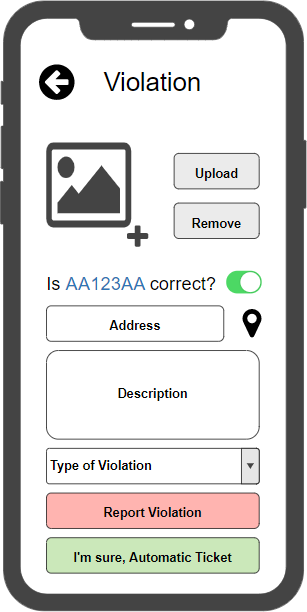
\includegraphics[width=0.6\linewidth]{images/mockups/violation}
	\caption{SafeStreets Violation page.}
	\label{fig:violation}
\end{figure}
\clearpage
\begin{figure}
	\begin{flushleft}
		\textbf{Unsafe Areas Page}:\\
		If the user wants to see which areas are the most subject to violations, an interface to search among all areas should be implemented.
	\end{flushleft}
	\centering
	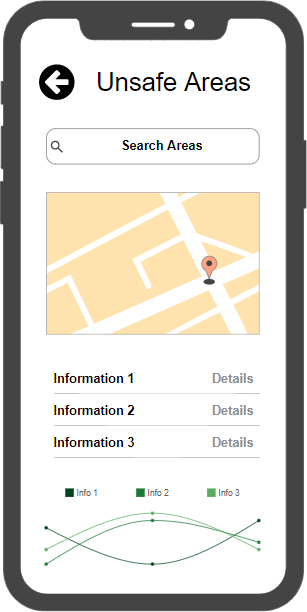
\includegraphics[width=0.6\linewidth]{images/mockups/areas}
	\caption{SafeStreets Unsafe Areas page.}
	\label{fig:areas}
\end{figure}
\clearpage
\begin{figure}
	\begin{flushleft}
		\textbf{Worst Drivers Page}:\\
		If the user wants to see which vehicles tends to not follow the city rules, an interface that shows this needs to be present in the application. A license plate search is better to be avoided.
	\end{flushleft}
	\centering
	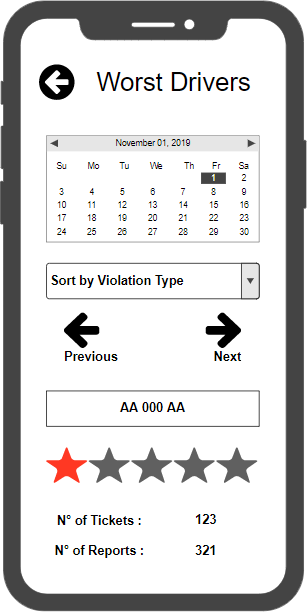
\includegraphics[width=0.6\linewidth]{images/mockups/vehicles}
	\caption{SafeStreets Worst Drivers page.}
	\label{fig:vehicles}
\end{figure}
\clearpage
\begin{figure}
	\begin{flushleft}
		\textbf{Statistics Page}:\\
		A complete page that exhibits all of SafeStreets data in a complete and detailed manner, that also enlightens SafeStreets effectiveness. 
	\end{flushleft}
	\centering
	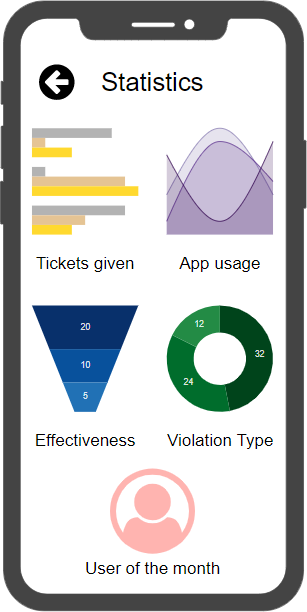
\includegraphics[width=0.6\linewidth]{images/mockups/statistics}
	\caption{SafeStreets Statistics page.}
	\label{fig:statistics}
\end{figure}
\clearpage
\begin{figure}
	\begin{flushleft}
		\textbf{User Profile Page}:\\
		If the user wants to change its profile picture or his password, if he wants to check his reports or to logout, he should be able to do all these things. 
	\end{flushleft}
	\centering
	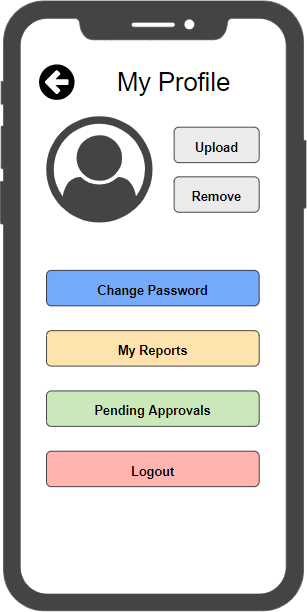
\includegraphics[width=0.6\linewidth]{images/mockups/profile}
	\caption{SafeStreets User Profile page.}
	\label{fig:profile}
\end{figure}
\clearpage